%%%%%%%%%%%%%%%%%%%%%%%%%%%%% Define Article %%%%%%%%%%%%%%%%%%%%%%%%%%%%%%%%%%
\documentclass{article}
%%%%%%%%%%%%%%%%%%%%%%%%%%%%%%%%%%%%%%%%%%%%%%%%%%%%%%%%%%%%%%%%%%%%%%%%%%%%%%%

%%%%%%%%%%%%%%%%%%%%%%%%%%%%% Using Packages %%%%%%%%%%%%%%%%%%%%%%%%%%%%%%%%%%
\usepackage{geometry}
\usepackage{graphicx}
\usepackage{amssymb}
\usepackage{amsmath}
\usepackage{amsthm}
\usepackage{empheq}
\usepackage{mdframed}
\usepackage{booktabs}
\usepackage{lipsum}
\usepackage{graphicx}
\usepackage{color}
\usepackage{psfrag}
\usepackage{pgfplots}
\usepackage{bm}
\usepackage{listings}
%%%%%%%%%%%%%%%%%%%%%%%%%%%%%%%%%%%%%%%%%%%%%%%%%%%%%%%%%%%%%%%%%%%%%%%%%%%%%%%

% Other Settings
\graphicspath{ {Images/} }
%%%%%%%%%%%%%%%%%%%%%%%%%% Page Setting %%%%%%%%%%%%%%%%%%%%%%%%%%%%%%%%%%%%%%%
\geometry{a4paper}

%%%%%%%%%%%%%%%%%%%%%%%%%% Define some useful colors %%%%%%%%%%%%%%%%%%%%%%%%%%
\definecolor{ocre}{RGB}{243,102,25}
\definecolor{mygray}{RGB}{243,243,244}
\definecolor{deepGreen}{RGB}{26,111,0}
\definecolor{shallowGreen}{RGB}{235,255,255}
\definecolor{deepBlue}{RGB}{61,124,222}
\definecolor{shallowBlue}{RGB}{235,249,255}
%%%%%%%%%%%%%%%%%%%%%%%%%%%%%%%%%%%%%%%%%%%%%%%%%%%%%%%%%%%%%%%%%%%%%%%%%%%%%%%

%%%%%%%%%%%%%%%%%%%%%%%%%% Define an orangebox command %%%%%%%%%%%%%%%%%%%%%%%%
\newcommand\orangebox[1]{\fcolorbox{ocre}{mygray}{\hspace{1em}#1\hspace{1em}}}
%%%%%%%%%%%%%%%%%%%%%%%%%%%%%%%%%%%%%%%%%%%%%%%%%%%%%%%%%%%%%%%%%%%%%%%%%%%%%%%

%%%%%%%%%%%%%%%%%%%%%%%%%%%% English Environments %%%%%%%%%%%%%%%%%%%%%%%%%%%%%
\newtheoremstyle{mytheoremstyle}{3pt}{3pt}{\normalfont}{0cm}{\rmfamily\bfseries}{}{1em}{{\color{black}\thmname{#1}~\thmnumber{#2}}\thmnote{\,--\,#3}}
\newtheoremstyle{myproblemstyle}{3pt}{3pt}{\normalfont}{0cm}{\rmfamily\bfseries}{}{1em}{{\color{black}\thmname{#1}~\thmnumber{#2}}\thmnote{\,--\,#3}}
\theoremstyle{mytheoremstyle}
\newmdtheoremenv[linewidth=1pt,backgroundcolor=shallowGreen,linecolor=deepGreen,leftmargin=0pt,innerleftmargin=20pt,innerrightmargin=20pt,]{theorem}{Theorem}[section]
\theoremstyle{mytheoremstyle}
\newmdtheoremenv[linewidth=1pt,backgroundcolor=shallowBlue,linecolor=deepBlue,leftmargin=0pt,innerleftmargin=20pt,innerrightmargin=20pt,]{definition}{Definition}[section]
\theoremstyle{myproblemstyle}
\newmdtheoremenv[linecolor=black,leftmargin=0pt,innerleftmargin=10pt,innerrightmargin=10pt,]{problem}{Problem}[section]
%%%%%%%%%%%%%%%%%%%%%%%%%%%%%%%%%%%%%%%%%%%%%%%%%%%%%%%%%%%%%%%%%%%%%%%%%%%%%%%

%%%%%%%%%%%%%%%%%%%%%%%%%%%%%%% Plotting Settings %%%%%%%%%%%%%%%%%%%%%%%%%%%%%
\usepgfplotslibrary{colorbrewer}
\pgfplotsset{width=8cm,compat=1.9}
%%%%%%%%%%%%%%%%%%%%%%%%%%%%%%%%%%%%%%%%%%%%%%%%%%%%%%%%%%%%%%%%%%%%%%%%%%%%%%%

%%%%%%%%%%%%%%%%%%%%%%%%%%%%%%% Title & Author %%%%%%%%%%%%%%%%%%%%%%%%%%%%%%%%
\title{Tarea 8}
\author{Juárez Torres Karla Romina}
%%%%%%%%%%%%%%%%%%%%%%%%%%%%%%%%%%%%%%%%%%%%%%%%%%%%%%%%%%%%%%%%%%%%%%%%%%%%%%%

\begin{document}
    \maketitle
  \section{Proporcionar una gráfica conexa $G(V, A)$ con al menos 17 vértices y al menos 35 aristas con pesos positivos en el intervalo $[1, 8] \cup \mathbb{Z}$ deberá haber al menos cuatro aristas de cada costo $c, c \in [1, 8] \cup \mathbb{Z}$. Aplicar los siguientes algoritmos a la gráfica dada $G$, ilustrando cómo van transformandose las estructuras y mostrando al final los valores de las etiquetas para cada vértice.}

V = {1, 2, 3, 4, 5, 6, 7, 8, 9, 10, 11, 12, 13, 14, 15, 16, 17}\\

A = {(1, 2), (1, 3), (1, 4), (2, 5), (2, 6), (3, 7), (3, 8), (4, 9), (4, 10), (5, 11), (5, 12), (6, 13), (6, 14), (7, 15), (7, 16), (8, 17), (9, 11), (9, 12), (10, 13), (10, 14), (11, 15), (11, 16), (12, 17), (13, 15), (13, 16), (14, 17), (15, 16), (16, 17), (1, 5), (2, 7), (3, 9), (4, 11), (5, 13), (6, 15)}\\

Para facilitar la visualización, la gráfica se representa en forma de lista de adyacencia:

\begin{lstlisting}[language = python]

1: [2, 3, 4, 5],
2: [1, 5, 6, 7],
3: [1, 7, 8, 9],
4: [1, 9, 10],
5: [2, 11, 12],
6: [2, 13, 14],
7: [3, 15, 16],
8: [3, 17],
9: [4, 11, 12],
10: [4, 13, 14],
11: [5, 9, 15, 16],
12: [5, 9, 17],
13: [6, 10, 15, 16],
14: [6, 10, 17],
15: [7, 11, 13, 16],
16: [7, 11, 13, 15, 17],
17: [8, 12, 14, 16]

\end{lstlisting}

\begin{enumerate}



\end{enumerate}

  \section{Sea $a$ una arista de peso mínimo de una gráfica $G = (V, A)$ con pesos
en las aristas.}

\subsection{Modificar tanto el Algoritmo Prim como el Kruskal para que
la arista $a$ siempre aparezca en el árbol generador de peso mínimo.}

\begin{itemize}
  \item  \textbf{Modificación del algoritmo de Prim:}\\
  Para garantizar que la arista $a$ siempre aparezca en el árbol generador de peso mínimo, podemos modificar el algoritmo de Prim de la siguiente manera:\\
  \begin{enumerate}
    \item Inicializar un conjunto vacío $MST$ para almacenar el árbol generador de peso mínimo.
    \item Inicializar una cola de prioridad $Q$ para almacenar los vértices y sus costos de conexión.
    \item Insertar el vértice inicial arbitrario en $Q$ con costo 0.
    \item Mientras $Q$ no esté vacío:
    \begin{enumerate}
      \item Extraer el vértice $v$ con el costo mínimo de $Q$.
      \item Si el vértice $v$ está en $MST$, ignorarlo y continuar al siguiente vértice en $Q$.
      \item Agregar la arista que conecta $v$ con su vértice padre en $MST$ al conjunto $MST$.
      \item Insertar todos los vecinos no visitados de $v$ en $Q$ con el costo correspondiente.
    \end{enumerate}
    \item Devolver $MST$.
  \end{enumerate}
  La modificación consiste en agregar una condición en el paso 4b para verificar si la arista que conecta el vértice $v$ con su vértice padre en el árbol generador de peso mínimo es la arista $a$. Si es así, se agrega al conjunto $MST$ sin verificar si el vértice $v$ está en $MST$.

  \item \textbf{Modificación del algoritmo de Kruskal:}\\
  Para asegurar que la arista $a$ siempre esté presente en el árbol generador de peso mínimo, podemos modificar el algoritmo de Kruskal de la siguiente manera:\\
  \begin{enumerate}
    \item Ordenar todas las aristas del grafo en orden no decreciente de peso.
    \item Inicializar un conjunto vacío $MST$ para almacenar el árbol generador de peso mínimo.
    \item Para cada arista $(u, v)$ en el orden de las aristas ordenadas:
    \begin{enumerate}
      \item Si la arista $(u, v)$ es la arista $a$, agregarla al conjunto $MST$.
      \item Si agregar la arista $(u, v)$ a $MST$ no crea un ciclo, agregarla a $MST$.
    \end{enumerate}
    \item Devolver $MST$.
  \end{enumerate}
  La modificación consiste en agregar una condición en el paso 3a para verificar si la arista actual es la arista $a$. Si es así, se agrega directamente al conjunto $MST$ sin realizar ninguna verificación adicional.
\end{itemize}

\subsection{Calcular el desempeño computacional de los algoritmos propuestos}

\begin{enumerate}
  \item \textbf{Modificación del algoritmo de Prim:}\\
  La modificación del algoritmo de Prim tiene un bucle principal que se ejecuta hasta que la cola de prioridad $Q$ esté vacía. En cada iteración, se extrae el vértice con el costo mínimo de $Q$ y se realizan operaciones constantes para verificar y agregar aristas al conjunto $MST$.\\

  La cola de prioridad $Q$ puede implementarse con una estructura de datos eficiente, como un montículo binario o un montículo de Fibonacci, lo que permite una inserción y extracción eficiente de elementos en tiempo logarítmico. Suponiendo que el tamaño del grafo es $V$ (número de vértices) y el número total de aristas es $E$, el tiempo de ejecución del algoritmo modificado de Prim es aproximadamente $O((V + E) \log V)$.
  \item \textbf{Modificación del algoritmo de Kruskal:}\\
  La modificación del algoritmo de Kruskal también tiene un bucle principal que itera sobre todas las aristas ordenadas. En cada iteración, se realiza una verificación constante para determinar si la arista actual es la arista $a$ y si agregarla crea un ciclo en el árbol generador.\\

  El ordenamiento de las aristas se realiza previamente y tiene un tiempo de ejecución de $O(E \log E)$ si se utiliza un algoritmo de ordenamiento eficiente, como el ordenamiento rápido (quicksort) o el ordenamiento por mezcla (merge sort). Luego, el bucle principal recorre todas las aristas en $O(E)$ y las operaciones constantes de verificación y agregado de aristas al conjunto $MST$ también se ejecutan en tiempo constante. En total, el tiempo de ejecución del algoritmo modificado de Kruskal es aproximadamente $O(E \log E)$.

\end{enumerate}

En términos generales, la complejidad asintótica del algoritmo modificado de Prim es mejor que la del algoritmo modificado de Kruskal, ya que $E$ puede ser mayor o igual que $V$, y en el peor de los casos, $E$ puede ser del orden de $V^2$. Sin embargo, es importante tener en cuenta que la eficiencia real de los algoritmos puede depender de factores adicionales, como la implementación específica, las estructuras de datos utilizadas y las características del grafo en particular.

  \section{Sea $G = (V, A)$ una gráfica conexa con pesos positovos sobnre las aristas. Supongamos que el costo de un árbol generador se define como el producto de los costos en las aristas.}
\subsection{Diseñar un algoritmo que determine el árbol generador de peso máximo, usando tal regla}

La modificación consiste en ordenar las aristas en orden decreciente en lugar de creciente.

\begin{enumerate}
  \item Ordenar todas las aristas del grafo en orden decreciente de peso.
  \item Inicializar un conjunto vacío $MST$ para almacenar el árbol generador de peso máximo.
  \item Para cada arista $(u, v)$ en el orden de las aristas ordenadas:
  \begin{enumerate}
    \item Si agregar la arista $(u, v)$ a $MST$ no crea un ciclo, agregarla a $MST$.
  \end{enumerate}
  \item Devolver $MST$.
\end{enumerate}

La modificación clave es el paso 1, donde las aristas se ordenan en orden decreciente en lugar de creciente. Esto asegura que se seleccionen primero las aristas más pesadas durante el proceso de construcción del árbol generador.


\subsection{Calcular el desempeño computacional del algoritmo propuesto, indicando las estructuras de datos usados para lograr tal desempeño.}

El desempeño computacional del algoritmo propuesto es similar al del algoritmo de Kruskal estándar, ya que implica ordenar las aristas y realizar operaciones de conjuntos disjuntos. A continuación se describen las estructuras de datos utilizadas y el desempeño esperado:

\begin{itemize}
  \item \textbf{Conjunto de vértices y aristas:} Se pueden utilizar estructuras de datos como matrices, listas de adyacencia o listas de aristas para almacenar los vértices y las aristas.
  \item \textbf{Estructura de datos de conjuntos disjuntos:} Para verificar si agregar una arista crea un ciclo, se requiere una estructura de datos eficiente para mantener y fusionar conjuntos disjuntos. La estructura de datos de Union-Find es comúnmente utilizada y tiene un desempeño de tiempo casi constante para las operaciones de unión y búsqueda de conjuntos.
\end{itemize}

El desempeño computacional del algoritmo propuesto es O(|E| log |V|), donde |V| es el número de vértices y |E| es el número de aristas en el grafo. Esto se debe principalmente al tiempo requerido para ordenar las aristas en orden decreciente. La estructura de datos de conjuntos disjuntos (Union-Find) también contribuye a la complejidad del algoritmo, pero su impacto es menor en comparación con el tiempo de ordenación de las aristas.



  \section{Elije $\lambda$ de tal modo que el siguiente sistema de ecuaciones tenga solución:
\begin{align*}
2x_1 - x_2 + x_3 + x_4 &= 1 \\
x_1 + 2x_2 - x_3 + 4x_4 &= 2 \\
x_1 + 7x_2 - 4x_3 + 11x_4 &= \lambda
\end{align*}}

Podemos representar el sistema de ecuaciones lineales utilizando matrices de la siguiente manera:

\[ AX = B \]

donde:

\[ A = \begin{bmatrix} 
2 & -1 & 1 & 1 \\
1 & 2 & -1 & 4 \\
1 & 7 & -4 & 11
\end{bmatrix} \]

\[ X = \begin{bmatrix} 
x_1 \\
x_2 \\
x_3 \\
x_4
\end{bmatrix} \]

\[ B = \begin{bmatrix} 
1 \\
2 \\
\lambda
\end{bmatrix} \]

Para que el sistema tenga solución, es necesario que la matriz de coeficientes A sea una matriz invertible, es decir, su determinante debe ser distinto de cero.

Entonces, para encontrar el valor de lambda que hace que el sistema tenga solución, podemos calcular el determinante de la matriz A y resolver la ecuación:

\[ \det(A) \neq 0 \]

Si el determinante de A es diferente de cero, entonces para cualquier valor de lambda, el sistema tendrá una única solución. Si el determinante es igual a cero, entonces existen valores particulares de lambda que hacen que el sistema tenga múltiples soluciones o no tenga solución.

Vamos a calcular el determinante de A:

\[ \det(A) = \begin{bmatrix} 
2 & -1 & 1 & 1 \\
1 & 2 & -1 & 4 \\
1 & 7 & -4 & 11
\end{bmatrix} \]

Utilizando operaciones elementales de filas, podemos simplificar la matriz A:

\[ \begin{bmatrix} 
2 & -1 & 1 & 1 \\
1 & 2 & -1 & 4 \\
1 & 7 & -4 & 11
\end{bmatrix} 
= \begin{bmatrix} 
2 & -1 & 1 & 1 \\
0 & 5 & -3 & 3 \\
0 & 8 & -5 & 10
\end{bmatrix} 
= \begin{bmatrix} 
2 & -1 & 1 & 1 \\
0 & 5 & -3 & 3 \\
0 & 0 & 1 & 4
\end{bmatrix} \]

Ahora, calculamos el determinante de la matriz resultante:

\[ \begin{bmatrix} 
2 & -1 & 1 & 1 \\
0 & 5 & -3 & 3 \\
0 & 0 & 1 & 4
\end{bmatrix} 
= 2 \cdot 5 \cdot 1 + (-1) \cdot (-3) \cdot 1 + 1 \cdot 3 \cdot 0 - 1 \cdot 5 \cdot 0 - (-1) \cdot 3 \cdot 0 - 2 \cdot (-3) \cdot 1
= 10 + 3 + 0 - 0 - 0 - (-6)
= 19 \]

El determinante de la matriz A es igual a 19. Como el determinante es diferente de cero, podemos concluir que para cualquier valor de lambda, el sistema tendrá una única solución.
Podemos representar el sistema de ecuaciones lineales utilizando matrices de la siguiente manera:

\[ AX = B \]

donde:

\[ A = \begin{bmatrix} 
2 & -1 & 1 & 1 \\
1 & 2 & -1 & 4 \\
1 & 7 & -4 & 11
\end{bmatrix} \]

\[ X = \begin{bmatrix} 
x_1 \\
x_2 \\
x_3 \\
x_4
\end{bmatrix} \]

\[ B = \begin{bmatrix} 
1 \\
2 \\
\lambda
\end{bmatrix} \]

Para que el sistema tenga solución, es necesario que la matriz de coeficientes A sea una matriz invertible.
Entonces
\[ \det(A) \neq 0 \]


Calculando el determinante de A:

\[ \det(A) = \begin{bmatrix} 
2 & -1 & 1 & 1 \\
1 & 2 & -1 & 4 \\
1 & 7 & -4 & 11
\end{bmatrix} \]

Simplificando la matriz A:

\[ \begin{bmatrix} 
2 & -1 & 1 & 1 \\
1 & 2 & -1 & 4 \\
1 & 7 & -4 & 11
\end{bmatrix} 
= \begin{bmatrix} 
2 & -1 & 1 & 1 \\
0 & 5 & -3 & 3 \\
0 & 8 & -5 & 10
\end{bmatrix} 
= \begin{bmatrix} 
2 & -1 & 1 & 1 \\
0 & 5 & -3 & 3 \\
0 & 0 & 1 & 4
\end{bmatrix} \]

Ahora, calculamos el determinante de la matriz resultante:

\[ \begin{bmatrix} 
2 & -1 & 1 & 1 \\
0 & 5 & -3 & 3 \\
0 & 0 & 1 & 4
\end{bmatrix} 
= 2 \cdot 5 \cdot 1 + (-1) \cdot (-3) \cdot 1 + 1 \cdot 3 \cdot 0 - 1 \cdot 5 \cdot 0 - (-1) \cdot 3 \cdot 0 - 2 \cdot (-3) \cdot 1
= 10 + 3 + 0 - 0 - 0 - (-6)
= 19 \]


El determinante de la matriz A es igual a 19. Como el determinante es diferente de cero.
Se puede ver como la tercera ecuación es redundante o no factible dado que es combinación de las dos primeras.
Concretamente es la combinacion de 3 veces la segunda fila menos la primera.

Siguiendo esto podemos decir que $\lambda=3(2)-1=5$.


  \section{Construir una di-gráfica de al menos 20 vértices y 30 arcos donde no donde si pueda
aplicarse el Algoritmo Topological Sort y muestre el resultado de aplicarlo.}

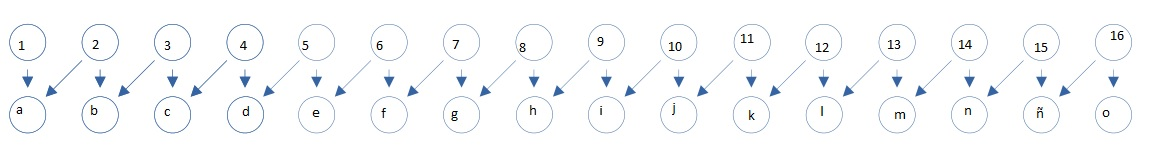
\includegraphics[scale=0.5]{2.jpg}

Resultado\\


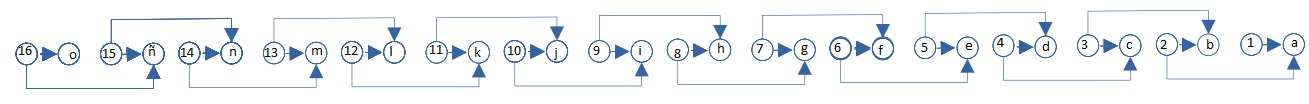
\includegraphics[scale=0.5]{3.jpg}



\end{document}

